\subsection{Single Responsibility Principle}

\compareTable
{\acrlong*{srp}}
{tab_convergence_srp_principle_summarized}
{\addEvalRow{\conv & \partconv & \partconv & \noconv}}

\subsubsection{\acrlong*{soc}}

The main goal of both \gls{srp} and \gls{soc} is to promote and encourage modularity, low
coupling, and high cohesion. While the definition has some differences, the two principles
can be regarded as practically interchangeable. Many examples in the Artifacts show a
strong alignment between \gls{srp} and \gls{soc}. To name one, an Expander should be able
to can perform multiple Tasks to complete the full instantiation of the Model. Each of
those Tasks can be implemented separately from each other. Figure \ref{fig_handlers}
illustrated some of the Tasks that are implemented in the Clean Architecture Expander
Artifact. The Code Listing \ref{list_entityexpander} is an example of one implementation
of such a Task \citecode{koks_expandentitieshandlerinteractor_2023}.

\begin{figure}[H]
    \centering
    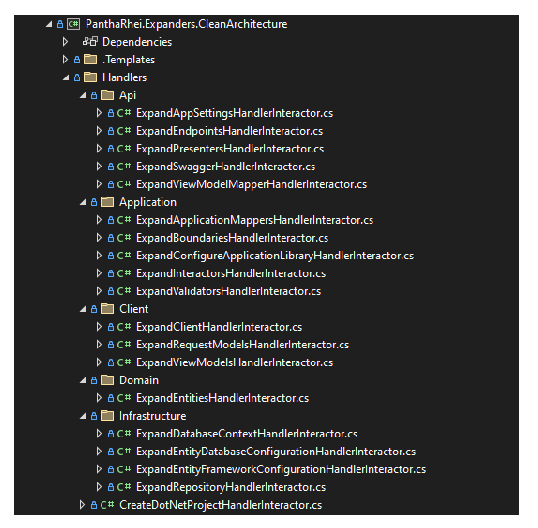
\includegraphics[width=0.6\textwidth]{figures/expander_handlers.pdf}
    \caption[handlers]{Each of the handlers handles an isolated part of the expanding process.}
    \label{fig_handlers}
\end{figure}

To sum up, \gls{srp} and \gls{soc} share the goal of organizing a software system into
modular components with specific \enquote*{responsibilities} or \enquote*{concerns}. This
convergence highlights the importance of encapsulating these responsibilities within a
software system.

\subsubsection{\acrlong*{dvt}} 

Although using \gls{srp} does not implicitly guarantees \gls{dvt}, it does support
\gls{dvt} by directing certain design choices. For example, both \gls{ca} and \gls{ns}
assign specific \gls{dto} objects to support specific use cases (Interactors or Tasks) or
to transfer (parts of) Data between architectural layers. \gls{ca} specifically assigned
\glspl{dto} and guidelines on where and when to use them. These are also applied in the
Artifact of this study as ResponseModels, RequestModels, and ViewModels
\parencites{koks_requestmodels_2023,koks_viewmodels_2023} \textcolor{red}{(TODO: Response
citation toevoegen)}. The separation of data structures specific to Use Cases minimizes
the impact of data structure changes by preferring stamp coupling over data coupling.
However, \gls{srp} is not a guaranteed measure for \gls{dvt}.

\subsubsection{\acrlong*{avt}} 

While \gls{srp} emphasizes limiting the responsibility of each module, it does not
explicitly require handling specific versions of use cases. Nevertheless, adhering to
gls{srp} can still indirectly contribute to achieving \gls{avt}. This can be achieved by
separating versions of Tasks into separate contracts, objects, or methods. The
manifestation described above, where different Tasks


by promoting the Law of
Demeter \footnote{\url{https://en.wikipedia.org/wiki/Law_of_Demeter}}, which encourages
modules to interact with each other only through well-defined interfaces. This approach
can minimize the impact of data structure changes, although it does not guarantee full
convergence with \gls{dvt}.

\subsubsection{\acrlong*{sos}} The convergence between \gls{srp} and the \gls{sos} theorem
is not as direct as with other theorems. \gls{srp} focuses on assigning a single
responsibility to each module but does not explicitly address state management.
Nevertheless, by following \gls{srp}, developers can create modules that manage their
state, which indirectly contributes to \gls{sos}.